\documentclass[a4paper,11pt]{report}
\usepackage[dvipsnames]{xcolor}
\usepackage{tikz}
\usepackage{pgfplots}
\pgfplotsset{compat=1.18}

\begin{document}
	
	\noindent % enlève indentation paragraphe
	
	\makebox[\textwidth][l]{%
		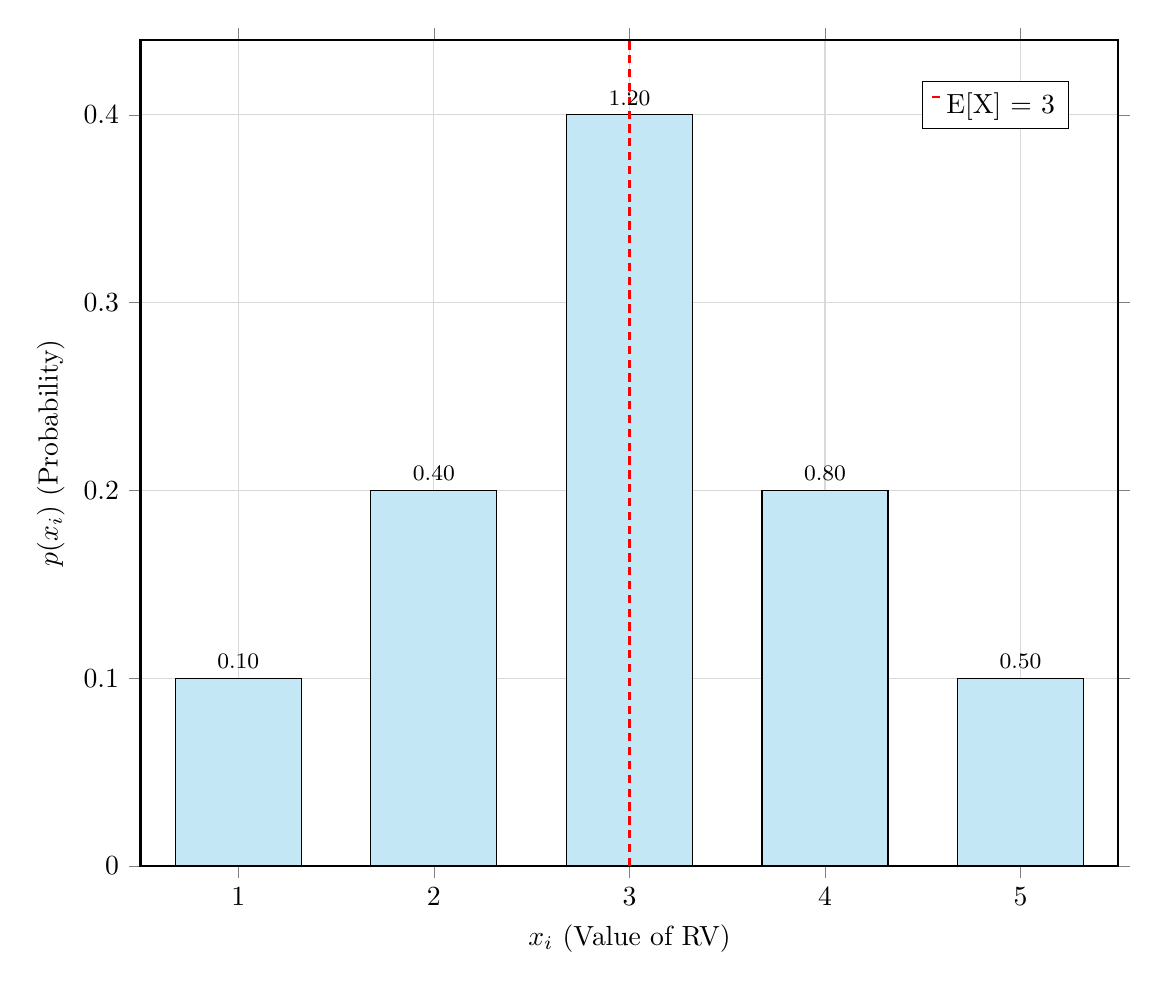
\begin{tikzpicture}
			\begin{axis}[
				ybar,
				width=14cm,           % largeur adaptée pour la marge
				bar width=1.6cm,
				xlabel={$x_i$ (Value of RV)},
				ylabel={$p(x_i)$ (Probability)},
				nodes near coords,
				point meta=explicit symbolic,
				every node near coord/.append style={
					font=\footnotesize,
					anchor=center,
					align=center,
					yshift=6pt,
				},
				xmin=0.5,
				xmax=5.5,
				ymin=0,
				xtick={1,...,5},
				ytick={0,0.10,0.20,0.30,0.40},
				grid=both,
				major grid style={gray!30},
				legend style={at={(0.95,0.95)}, anchor=north east},
				legend cell align=left,
				enlarge x limits=false,
				axis line style={black, line width=0.8pt},
				tick align=outside,
				%shift only axis, % <-- on enlève cette ligne pour éviter plantage
				%axis on top,      % <-- aussi supprimée pour la stabilité
				]
				
				\addplot[
				fill=SkyBlue!50,
				draw=black,
				ybar,
				forget plot
				] table[x=x, y=y,meta=label, row sep=\\] {
					x y label \\
					1 0.10 {0.10} \\
					2 0.20 {0.40} \\
					3 0.40 {1.20} \\
					4 0.20 {0.80} \\
					5 0.10 {0.50} \\
				};
				
				\draw[densely dashed, thick, red]
				(axis cs:3,0) -- (axis cs:3,0.45);
				
				\addplot[
				red,
				densely dashed,
				thick,
				mark=none,
				legend image code/.code={
					\draw[red, densely dashed, thick] (0cm,0.1cm) -- (0.1cm,0.1cm);
				}
				] coordinates {(0,0) (0,0)};
				\addlegendentry{E[X] = 3}
				
			\end{axis}
		\end{tikzpicture}
	}
	
\end{document}
